\documentclass[11pt]{article}
\usepackage[margin=0.55in]{geometry}
\usepackage{graphicx,caption,amsmath,float}
\usepackage[colorlinks=true,urlcolor=blue!50!black]{hyperref}
\captionsetup{font=footnotesize,labelfont=bf,skip=2pt,width=0.90\textwidth}
\pagestyle{empty}
\renewcommand{\textfraction}{0.05}
\renewcommand{\bottomfraction}{0.75}
\renewcommand{\topfraction}{0.9}
\renewcommand{\floatpagefraction}{0.6}
\setlength{\parskip}{2pt}
\setlength{\parindent}{0pt}
\setlength{\textfloatsep}{5pt plus 2pt minus 2pt}
\setlength{\intextsep}{5pt plus 2pt minus 2pt}
\setlength{\floatsep}{5pt}


\begin{document}


\begin{center}
{\large\bfseries\setlength{\baselineskip}{1.05\baselineskip}
Moneyball your MLB Pitching Staff across Roles with FIP\_Pyth\_WinRate and
FIP\_Pyth\_WL: ML-Validated, All-Role Scalable Measures of Pitcher Win Output per
Opportunity (Arbitrage) \& Pitching's Share of Winning\par}\vspace{3pt}\par
{\small  \textbullet\ Baseball Track}
\end{center}

\textbf{Introduction.} Pitcher evaluation has advanced from win-loss record, or saves and holds in relief, through earned run average (ERA), Fielding Independent
Pitching (FIP), and pitcher Wins Above Replacement (pWAR). This progression sacrificed the team-aligned output unit per opportunity. No existing measure provides a win-rate (loss-rate) \emph{per pitching opportunity}, and relief pitchers were never evaluated in an apples-to-apples framework. Win-Loss, Saves, and Holds are 3 different measures with distinct units, none being high-signal or team-aligned. Then, the founding \emph{Moneyball} question (\emph{Which inputs does the market misprice?}) has never been answerable across a pitching-staff. Even $pWAR$ does not balance a pitcher's opportunities with their success-rate. \textbf{ML ridge-regression} shows that a 2-WAR middle-reliever (closer, starter) supports a win-rate of 0.589 (0.615, 0.511), with IP-differential being the confound. Using tools from ML and game theory, we develop \texttt{FIP\_Pyth\_WinRate} and \texttt{FIP\_Pyth\_WL}, which map pitcher-$FIP$, league-average $FIP$, and league-average unearned run-rate to an MLB-optimized Pythagorean win-function (contest success function in game theory) to express any pitcher's output as an advanced expected win-rate per 9-inning opportunity and an advanced win-loss record, in equivalent terms for all pitching-roles. The measures also meritoriously divide/assign partial-wins to pitchers appearing in a game without confounds like game-innings pitched, run-support, or starter-designation. 

\vspace{6pt}
\noindent\textbf{Methods.} We estimate the following equations and fit them onto cross-role pitcher win-output and marginal-revenue product 3-D surfaces.
\vspace{-8pt}

{\setlength{\abovedisplayskip}{0pt}\setlength{\belowdisplayskip}{3pt}
\begin{small} \begin{align}
\text{W\%}_{\text{team}}=\frac{RS^{\gamma}}{RS^{\gamma}+RA^{\gamma}},\qquad
w_{p}=\frac{(F^{*}+u)^{\gamma}}{(F^{*}+u)^{\gamma}+(\mathrm{FIP}_{p}+u)^{\gamma}},\qquad
(W_{p},L_{p})=\bigl(G_{p}\,w_{p},\; G_{p}(1-w_{p})\bigr)
\end{align}
\end{small}}

\noindent $W\%_{team}$ is team Pythagorean expected-win\%; $w_{p}$ is \texttt{FIP\_Pyth\_WinRate} and
$(W_{p},L_{p})$ is \texttt{FIP\_Pyth\_WL}, $RS$ and $RA$ are runs scored and allowed per game,
$\gamma=1.83$, $\mathrm{FIP}_{p}$ is pitcher $p$'s $FIP$, $u$ the league
unearned-run rate, $F^{*}$ the win-neutral FIP at which a staff breaks even, and
$G_{p}=\mathrm{IP}_{p}/9$ their nine-inning opportunities. The first equation in (1) estimates $\gamma$ from \textbf{nonlinear Weibull regression}. The second maps the optimal Pythagorean-wins function to the individual-pitcher FIP-level. It asks the pitcher's win-rate per 9-innings versus league-average opposing-FIP and a league-average unearned run-rate across teams. The third equation scales this win (loss) rate by full-game equivalents pitched to develop a valid W-L record for any pitcher. 

\begin{figure}[H]
\centering
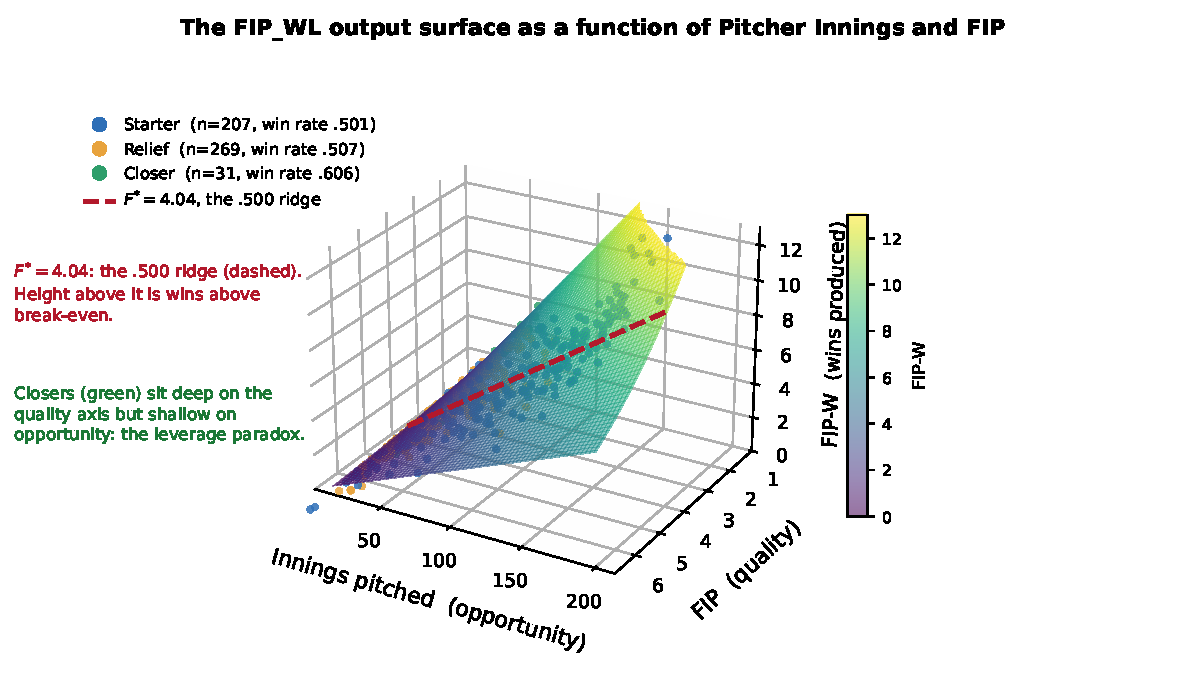
\includegraphics[height=60mm]{absfig1 (2).pdf}\hfill
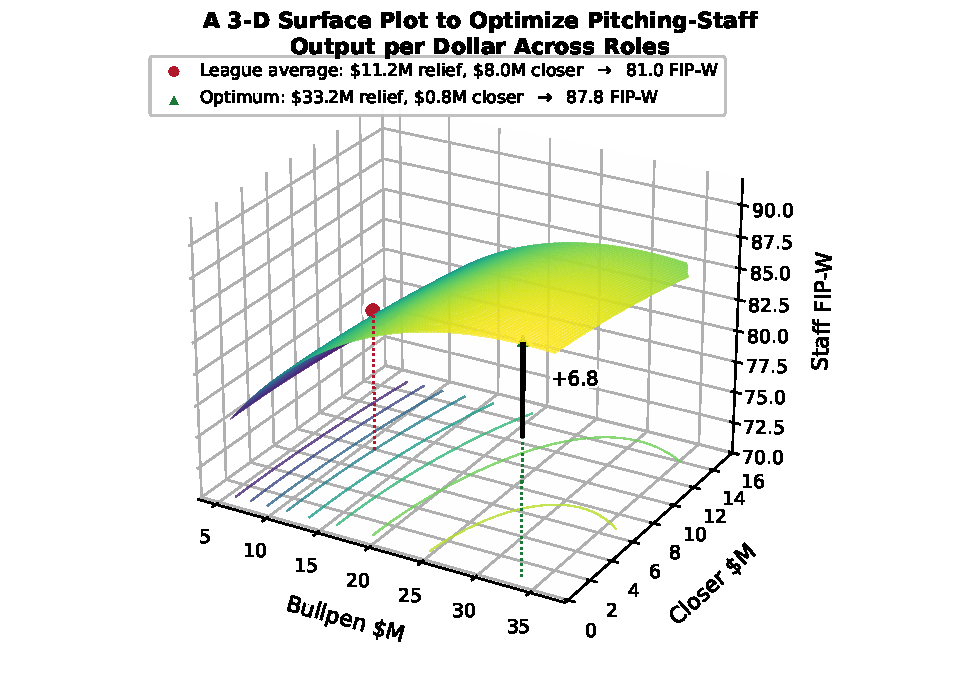
\includegraphics[height=60mm]{absfig3 (2).pdf}
\vspace{-2pt}
\caption{\textbf{Left:} every 2026 pitcher on a single surface --- quality against opportunity,
elevation in wins --- with the dashed red ridge marking the win-neutral anchor at which a pitcher is
exactly break-even. Starters, relievers and closers are graded on the same curve. \textbf{Right:}
staff wins over bullpen and closer spending on a fixed \$53.2M payroll, the rotation absorbing the
residual; the club climbs from $81$--$81$ to $88$--$74$.}
\end{figure}

\textbf{Results.} Estimating on complete \emph{Baseball Reference} MLB pitcher-data for 2023---2026, we validate and apply the measures using ML and statistical-learning models. We \textbf{ridge regress} team-season wins on \texttt{FIP\_Pyth\_WL}-estimated wins, runs the defense saved or surrendered, and runs the offense scored. Whereas direct FIP-measures fail to aggregate to a 0.5 implied league-average win-rate by \textbf{Jensen's inequality}, \texttt{FIP\_Pyth\_WinRate} does given its optimized-Pythagorean win-calibration. An MLB team-season decomposes into five win-inputs explaining \textbf{98.8\,\% of variation in winning}: \textbf{offense at 37.9\,\%}, sequencing of baserunners and outs at
\textbf{26.3\,\%}, \textbf{FIP-wins at 20.9\,\%}, fate of balls in play at 12.3\,\%, and fielding errors at 1.4\,\%. Chance sequencing, or random-clustering of on-base events, changes ERA. It is sequencing, not fielding, that ERA mostly mistakes for pitching. \texttt{FIP\_Pyth\_WinRate} and \texttt{FIP\_Pyth\_WL} isolate fielding, sequencing, and pitching. Pitching, at 20.9\,\%, is significantly more win-productive than fielding (e.g., in \textbf{bootstrap resamples}).



\textbf{Ridge}, \textbf{random forest}, and \textbf{gradient boosting} train on the 2023-to-2024 and 2024-to-2025 transitions and test on the 2025-to-2026 transition. \texttt{FIP\_Pyth\_WinRate} is \textbf{twice as persistent across season as ERA}, demonstrating a substantial signal-to-noise/skill-to-noise gain. $\texttt{FIP\_Pyth\_WinRate}$ permutation importance on \textbf{held-out seasons} ranks first against twelve rival-inputs, \textbf{4 times stronger than ERA}, in picking best-available pitchers of 2025-26 blind. \textbf{Conformal quantile-boosting} gives each pitcher a projection-range, so signing is judged on downside, midpoint, and upside. Lastly, \textbf{decision-weighted boosting} fits wins on runs-allowed and confirms the team-optimized Pythagorean exponent holds at individual pitcher-level.

\textbf{Conclusion.} After calibrating/validating of the measures as pushing the MLB analytic-frontier, we apply them for the first known apples-to-apples \emph{Moneyball} analysis of the whole pitching-staff. Merging 819 individual 2026 contracts, closers earn a median \$7.50M against \$0.80M for other
relievers on fewer innings, \textbf{\$21M per marginal win}. Crossing role with service class, a win costs
\$0.13M from a pre-arbitration starter, \$0.39M from a pre-arbitration reliever, \$0.90M from a
veteran reliever, \$3.16M from a veteran starter, and \$3.32M from a veteran closer--a
\textbf{twenty-six-fold spread} in which class dominates role and the role effect reverses. % ===========================================================================
% Plain-language version of the closing sentence. Same numbers, no shorthand.
%
% What the jargon meant:
%   "closer walks at the minimum"  -> do not re-sign him; fill the spot with a
%                                     league-minimum pitcher ($8.00M -> $0.78M)
%   "trading the rotation down"    -> cheaper #4 and #5 starters
%                                     ($6.80M -> $3.85M per starting spot)
%   "tripling spending per place"  -> per ROSTER SPOT, not in total
%                                     ($1.60M -> $4.74M per relief spot)
%   "better relievers, not more"   -> same 7 spots, same innings, better arms
%   "81-81 staff"                  -> the team record implied by the pitching,
%                                     with offense and defense held at average
%
% 112 words.
% ===========================================================================

We conclude that a league-average team can go from 81-81 to 88-74 in expectation without spending any more money,
by changing who fills three sets of roster spots. First, the team should not re-sign its closer, and instead give the role to the best-available pre-arbitration reliever at a $\$7^+$M savings. Second, the team should replace its fourth and fifth starters with cheaper ones, cutting average pay for those two spots from \$6.80M to \$3.85M.
Third, the team spends everything it freed up, roughly \$22M, on its seven middle-relief spots, raising pay
per spot from \$1.60M to \$4.74M. The bullpen throws the same number innings with better pitchers. On
the same \$53.2M payroll, the record implied by the pitching improves from \textbf{81--81 to 88--74}. The strategy is win-positive in $80$\,\% of \textbf{200{,}000}
simulated seasons, and $92.7$\,\% cumulatively if run for three winters, as the gain accumulates
linearly while its dispersion grows with the square root of seasons.





\begin{figure}[H]
\centering
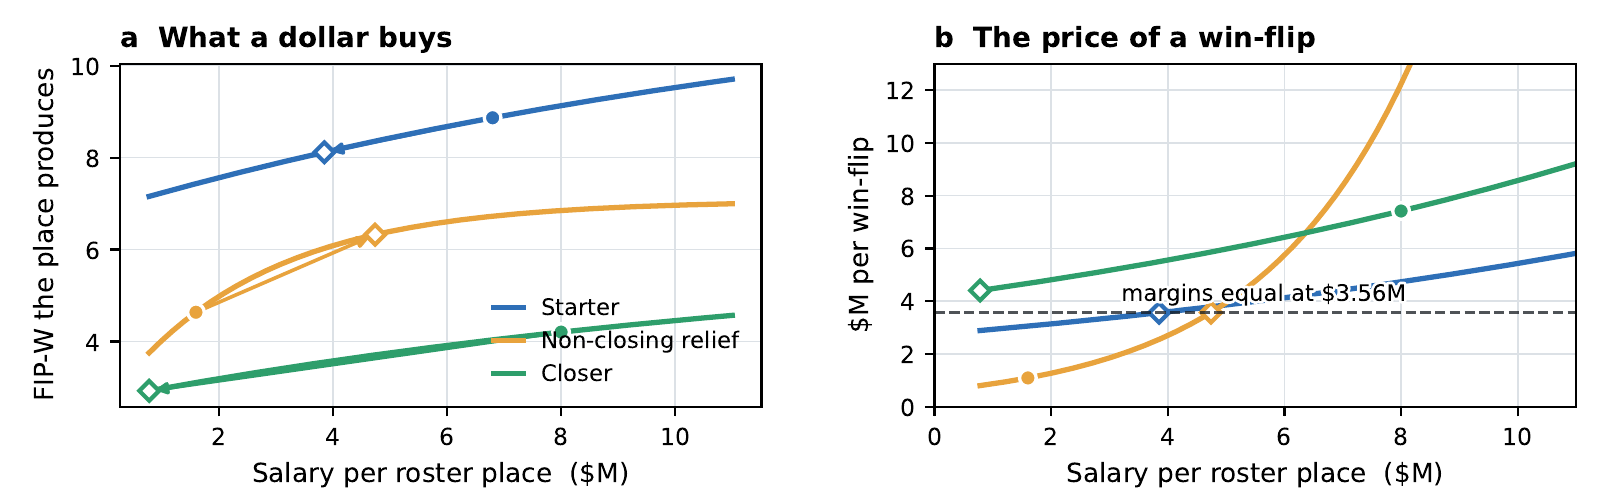
\includegraphics[width=0.95\textwidth]{fig_marginal_sm (1).png}
\vspace{-2pt}
\caption{\textbf{(a)} What a dollar buys at each role: the concave gradients fitted to individual
2026 contracts. \textbf{(b)} The resulting marginal cost of flipping one loss into one win --- \$1.09M
in the bullpen, \$4.36M in the rotation, \$7.42M at closer --- with a club buying until the three
margins meet. Circles mark the league-average contract at each role, diamonds the reallocated
position.}
\end{figure}

\end{document}